
\documentclass{article}

% Language setting
% Replace `english' with e.g. `spanish' to change the document language
\usepackage[dvipsnames]{xcolor}
\usepackage[english]{babel}
\usepackage{cite}  % If you want to use numerical citations
\usepackage{subcaption}
\usepackage{float}
\usepackage[nogroupskip, acronym, toc]{glossaries} % Package for glossary
\usepackage{subcaption}
\usepackage{multirow}
\usepackage{comment}
\usepackage{pgfplots}
\usepackage{pdfpages}
\usepackage{listings}
\usepackage[nobiblatex]{xurl}
\usepackage{amsmath}




\lstdefinestyle{mystyle}{
    backgroundcolor=\color{White},   
    commentstyle=\color{Green},
    keywordstyle=\color{RedOrange},
    numberstyle=\tiny\color{Gray},
    stringstyle=\color{Plum},
    basicstyle=\ttfamily\footnotesize,
    breakatwhitespace=false,         
    breaklines=true,                 
    captionpos=b,                    
    keepspaces=true,                 
    numbers=left,                    
    numbersep=5pt,                  
    showspaces=false,                
    showstringspaces=false,
    showtabs=false,                  
    tabsize=2
}

\lstset{style=mystyle}

\makeglossaries

\newacronym{scm}{SCM}{Smart Composite Manufacturing}
\newacronym{cad}{CAD}{Computer Aided Design}
\newacronym{mCT}{$\mu$CT}{Microcomputed Tomography }
\newacronym{cot}{CoT}{Cost of Transport}
% Set page size and margins
\usepackage[a4paper,top=2cm,bottom=2cm,left=3cm,right=3cm,marginparwidth=1.75cm]{geometry}

% Useful packages
\usepackage{amsmath}
\usepackage{amssymb}
\usepackage{graphicx}
\usepackage{caption}
\usepackage{subcaption}
\usepackage[colorlinks=true, allcolors=blue]{hyperref}
\usepackage{upgreek}
\usepackage[nottoc,notlot,notlof]{tocbibind}

\pagenumbering{gobble}


\title{

\includegraphics[scale=0.15]{images/University_of_Edinburgh_ceremonial_roundel.svg.png}

\vspace{72pt}

\hline 


\vspace{12pt}

%\Large{ }
\Large{Advanced Dynamics and Applications 5 Technical Review Report}

\vspace{12pt}
\LARGE{\textbf{Mitigation of EOV via non-linear regression in Wind Turbines}} 

%From e-waste to robotics: characterising and upcycling e-waste into educational robot demonstrators}

\vspace{12pt}

%\Large{Supervisor: Dr. Parvez Alam}


\vspace{12pt}

\hline

\vspace{36pt}

\Large{
Will Lewis

Conrad Thomson

Yordan Tsvetkov
}

}

\begin{document}


\maketitle

\pagebreak

\tableofcontents

\pagebreak

\printglossary[type=\acronymtype]

\pagebreak

\section{Technical Review}

\subsection*{Abstract (100-150 words)}
\label{Abstract}
Ask if abstract is in the page limit!!!

A summary of the research question, methods and main general findings.

- paper: analyses the effect of the number of considered DSFs
- paper: method proposed for dealing with a large number of outliers


\pagebreak

\pagebreak
\pagenumbering{arabic}
\subsection{Introduction and Motivation ($\approx$1 page)}
\label{Introduction}

\subsection{Theoretical Fundamentals and Methodology ($\approx$1.5 page)}
\textbf{1 page Yordan (book), 0.5 pages Will (paper)}

\subsection{Experimental validation ($\approx$1 page)}
\textbf{1 page Conrad}

\textit{- Take about the errors encountered in the experimental data, not on the limits outside of the data!}

The analysis on the impact of EOVs on selected DSFs situated at nodes on the wind turbine blades takes a divergent approach, considering both implicit and explicit procedures as the methodology underlying the multi-variate non-linear regression. Implicit methods, while computationally economical, functions by filtering data points by their degree of variability, which signifies the contribution of EOVs on the data. By defining a threshold level of variance to indicate the point at which EOVs (such as temperature) must have a disproportionate effect on the result in comparison to physical damage. However, this absolutist methodology of completely negating outlying data points comes with an inherently attached downside. 

\subsection{Discussion and Innovations ($\approx$0.5 pages)}
\textbf{0.5 pages Will}

\textit{How does this paper expand on previous work in the field}
\begin{itemize}
    \item Are their models more refined?
    \item More intelligent algorithms?
    \item Identification of pertinent variables and concepts ignored in other papers etc.
\end{itemize}


\subsection{Conclusions and Limitations ($\approx$1 page total, 0.5 pages each)}
Summary of the work done, what can be expanded upon, what should be done as further study, where can it be applied. 

- paper: limited training data - \textit{Consequently, a limitation is introduced into this work where the undamaged and damaged states may have experienced different ranges of conditions since the experiment lasted 4 months. As a result, the models created from the undamaged data might not transfer properly for the damaged data.} \cite{paper_ref20}

- paper: large number of outliers (end of p. 1250)

\pagebreak

\section{Technical Simulation}

\renewcommand{\thesubsection}{Q.\arabic{subsection}}

\large\textbf{Preamble}\medskip\\
\label{preamble}

Following from the evaluation of the study undertaken to identify and predict DSFs present on wind turbine blades subject to EOVs, this underlying theory shall now be extended to a numerical problem concerning a cantilever beam. Figure \ref{fig:beam} represents a proprietary structural beam member, subject to potential deterioration inflicted by longitudinal forced vibration. The beam is fixed at one end, and has been outfitted with an equidistant array of accelerometers, effectively subdividing the structure into three finite elements, connected by four nodes.\medskip\\
While this is a multiple-degree-of-freedom system, it is sufficiently simple to perform analytical dynamic predictions before employing the use of programmatic tools and FEM software for accurate results and theoretical validation. Throughout this numerical analysis, the tools used were Python3, which is host to the industry-leading scientific libraries of Numpy and Scipy, which aid tremendously in data analysis and matrix manipulation. In addition, the JavaScript library D3.js was used for data visualisation on display in all 2D graphs present in this report. Ultimately, the FEM software \textit{Abaqus/SimScale [yet to decide which one to use]} was utilised to validate and verify all results generated. A collective consensus was achieved through the progressive use of pen-on-paper mathematical reasoning, followed by efficient data analysis using robust programming languages, and finalising verification by performing thorough simulations with industrial-grade FEM software. The unison shown by three independent methodologies is testament to the validity of the results described qualitatively and quantitatively in this report.\medskip\\

\large\textbf{System Configuration}
\label{system_config}

\begin{figure}[h!]
    \centering
    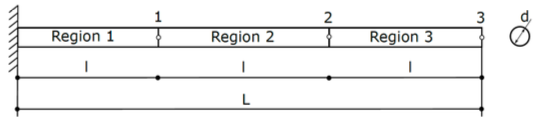
\includegraphics[width=0.75\textwidth]{images/cantBeam.png}
    \caption{Graphical representation of the cantilever beam and defined regions}
    \label{fig:beam}
\end{figure}

As with any physical structure, this cantilever beam can be abstracted into its fundamental constituents defining its complete dynamic behaviour. By deconstructing the beam into a coupled series of masses, springs and dampers, the equations of motion can be found through the use of a Free Body Diagram representation, governed by the classical laws of motion. The free body diagram is shown in Fig. \ref{fig:fbd}.\medskip\\

\begin{figure}[h!]
    \centering
    \includegraphics[width=0.75\textwidth]{images/}
    \caption{Free Body Diagram Model}
    \label{fig:fbd}
\end{figure}

\subsection{Equations of Motion}
\label{1_eom}

By separating the masses and balancing forces, the systems' equations of motions are derived, omitting any external forces/torques at this stage. It is assumed that the beam is homogeneous along its length in both its geometric and material properties. The corollary to this assumption is the equivalence in mass, stiffness, and damping in each of the three masses, springs, and dampers, respectively. This is due to the equivalent length, cross-sectional area, density and strength of each element. Defining $l = L/n$, the elemental mass and stiffness can be described by:

\begin{gather}
    m_i = \frac{\rho A l}{2} ,\quad i\in{[1, 2]} \\
    m_3 = \rho Al \\
    k_i = k = \frac{E A}{l} ,\quad\forall i
\end{gather}

Note the elemental mass represents the lumped mass; that is, each discrete element's dynamical \textit{effective mass} contributing to its inertia. In the analytical model, both masses $m_1\ \text{and}\ m_2$ are supported by springs on both sides, distributing vibrational energy between their immediate surrounding elements (in this system, transferred in equal part to both supporting springs).  Conversely, at the free end $m_3$ retains its actual mass as its effective dynamic mass, as it is supported by only one spring and can therefore only transfer its energy through the spring.\medskip\\
The springs all share an equivalent stiffness by extension of the beam's homogeneity.\medskip\\
Three degrees of freedom yield three equations of motion, as described below.

\begin{equation}
    \begin{aligned}
        m_1\ddot{x_1} &+ c_1\dot{x_1} + k_1\dot{x_1} - c_2(\dot{x_2} - \dot{x_1}) - k_2(x_2 - x_1) = 0 \\
        m_2\ddot{x_1} &+ c_2(\dot{x_2} - \dot{x_1}) + k_2(x_2 - x_1) - c_3(\dot{x_3} - \dot{x_2}) - k_3(x_3 - x_2) = 0 \\
        m_3\ddot{x_1} &+ c_3(\dot{x_3} - \dot{x_2}) + k_3(x_2 - x_1) = 0 \\
    \end{aligned}
\end{equation}

\noindent This is a linear system of equations, which can be translated into matrix form in accordance with the generalised ODE governing mass-spring-damper mechanical systems:

\begin{equation}
    \mathbf{M}\Vec{\ddot{x}} + \mathbf{C}\Vec{\dot{x}} + \mathbf{K}\Vec{x} = \mathbf{0}
\end{equation}

\noindent Collecting like terms and assembling the coupled equations of motions results in the following linear system.

\begin{multline}
    \begin{bmatrix}
        m_{1} & \cdots & 0 \\
        \vdots & m_{2} & \\
        0 & & m_{3}
    \end{bmatrix}
    \left\{ \begin{array}{c}
         \ddot{x_1} \\
         \ddot{x_2} \\
         \ddot{x_3}
    \end{array} \right\}
    +
    \begin{bmatrix}
        2c_{1} & -c_{2} & 0 \\
        -c_{1} & 2c_{2} & -c_{3} \\
        0 & -c_{2} & c_{3}
    \end{bmatrix}
    \left\{ \begin{array}{c}
         \dot{x_1} \\
         \dot{x_2} \\
         \dot{x_3}
    \end{array} \right\} \\
    + \begin{bmatrix}
        2k_{1} & -k_{2} & 0 \\
        -k_{1} & 2k_{2} & -k_{3} \\
        0 & -k_{2} & k_{3}
    \end{bmatrix}
    \left\{ \begin{array}{c}
         x_1 \\
         x_2 \\
         x_3
    \end{array} \right\}
    = \mathbf{\vec{d}}
\end{multline}


\pagebreak
\subsection{The Eigenvalue Problem: Deriving Natural Frequencies \& Mode Shapes}
\label{2_natFreq_mode}

To progress with the structural analysis, the natural frequencies and corresponding mode shapes are sought. Natural frequencies are system properties, independent of applied forces. Cyclic forces and impact loads \textit{can} alter the structure's natural frequencies, but only through deforming or damaging the system, effectively transforming it into a different system entirely. Analysing the beam with the properties measured in its static state, the natural frequencies are first determined by evaluating the eigenvalues of of the state matrix $\mathbf{A}$. Subsequently, the mode shapes are inferred from the eigenvectors generated from this eigen-analysis. The \textbf{Eigenvalue problem} is formulated as below.
\begin{equation}
    ({\mathbf{A}} - \lambda_n\mathbf{I})\mathbf{v}_n = 0
\end{equation}
This formula relies of the assumption of harmonic motion. In free vibration,
\begin{equation}
    \Vec{x} = \left\{ \begin{array}{c}
         x_1 \\
         x_2 \\
         x_3
    \end{array} \right\} e^{j\omega t}.
\end{equation}
In this analysis, 

\pagebreak

\bibliographystyle{ieeetr}


\bibliography{bibliography}
\end{document}